\documentclass[11pt,xcolor=svgnames]{beamer}
\usepackage{dsfont,natbib,setspace,changepage,multirow}
\mode<presentation>

% fonts

% replaces beamer foot with simple page number
\setbeamertemplate{navigation symbols}{}
\setbeamercolor{frametitle}{fg=black}
\setbeamerfont{frametitle}{series=\bfseries}
\setbeamerfont{frametitle}{size=\normalsize}
\newcommand{\theme}{\color{Maroon}}

\setbeamertemplate{footline}{
   \raisebox{5pt}{\makebox[\paperwidth]{\hfill\makebox[20pt]{\color{gray}\scriptsize\insertframenumber}}}}

\graphicspath{{../graphs/}}

% colors
\newcommand{\bk}{\color{black}}
\newcommand{\rd}{\color{red}}
\newcommand{\fg}{\color{ForestGreen}}
\newcommand{\bl}{\color{blue}}
\newcommand{\gr}{\color{gray}}
\newcommand{\sg}{\color{DarkSlateGray}}
\newcommand{\br}{\color{SaddleBrown}}
\newcommand{\nv}{\color{Navy}} 
\setbeamercolor{itemize item}{fg=gray}

% common math markups
\newcommand{\bs}[1]{\boldsymbol{#1}}
\newcommand{\mc}[1]{\mathcal{#1}}
\newcommand{\mr}[1]{\mathrm{#1}}
\newcommand{\bm}[1]{\mathbf{#1}}
\newcommand{\ds}[1]{\mathds{#1}}
\newcommand{\indep}{\perp\!\!\!\perp}

% spacing and style shorthand
\setstretch{1.1}

% shorthand
\newcommand{\sk}{\vspace{.5cm}}
\newcommand{\R}[1]{{\tt \nv #1}}
\newcommand{\til}{{\footnotesize$\bs{\stackrel{\sim}{}}$}}
\DeclareSymbolFont{extraup}{U}{zavm}{m}{n}
\DeclareMathSymbol{\vardiamond}{\mathalpha}{extraup}{87}

\begin{document}

\setcounter{page}{0}
{ \usebackgroundtemplate{
\includegraphics[height=\paperheight]{phoenix}}
\begin{frame}[plain]
\begin{center}


{\bf \Large [2] Big Data: Regression}

\vskip 1.5cm
Matt Taddy, University of Chicago Booth School of Business

\vskip .2cm
\texttt{faculty.chicagobooth.edu/matt.taddy/teaching}


\end{center}
\end{frame} } 


\begin{frame}
{[2] \theme  Regression}


Regression through  linear models, and how to do it in R.

\vskip .25cm
Interaction, factor effects, design ({\tt model}) matrices.

\vskip .25cm
{\bk Logistic Regression:} an essential BD tool.

\vskip .25cm
{\bk Estimation:} Maximum Likelihood and Minimum Deviance


\sk{\gr 
Much of this  should be review, but  emphasis will be different.}

\end{frame}


\begin{frame}
{\theme Linear Models}

Many problems in BD involve a response of interest
(`{\theme y}')\\ and a set of covariates (`{\theme \bf x}') to
be used for prediction.

\sk
A general tactic is to deal in averages and lines.  \\
{We'll model the {\theme
  conditional mean} for {\theme y given {\bf x}},}
{\large\[
\ds{E}[~ y \mid \bm{x} ~] = f( \bm{x}'\bs{\beta} )
\]}


$\bm{x} = [1, x_1, x_2,\ldots x_p]$  is your vector of
    covariates.\\
\vskip .2cm
$ \bs{\beta} = [\beta_0, \beta_1, \beta_2, \ldots \beta_p]$ are the corresponding
coefficients.\\
\vskip .2cm
The product is $\bm{x}'\bs{\beta}  = \beta_0 +
x_1\beta_1 + x_2\beta_2 + \ldots + x_p\beta_p$.
\vskip .2cm
\gr For notational convenience we use $x_0=1$ for the intercept.

\end{frame}


\begin{frame}

{\bf {\nv Marginal}
and {\nv conditional} distributions}

\vskip .25cm
~~~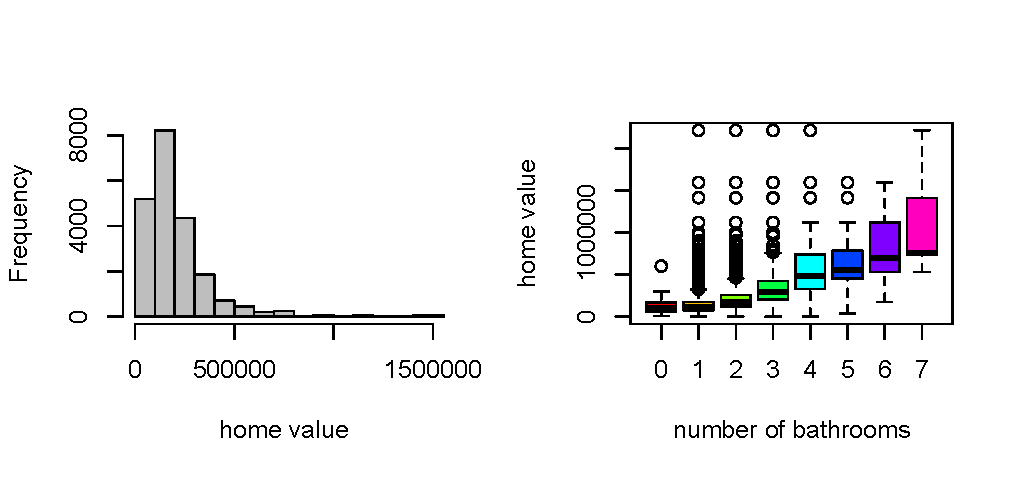
\includegraphics[width=4in]{../graphs/homes_margvcnd}

{\sg On the left, all of the homes are grouped together.\\
On the right, home prices are grouped by {\small {\tt \#}} baths.}

\sk The {\theme marginal mean} is a simple number.\\ The {\theme conditional
  mean} is a function that depends on covariates.

\vskip .25cm
The data is {\theme distributed} randomly around these means.
\end{frame}


\begin{frame}


In a [Gaussian] linear regression,
\vspace{-.25cm}
{\large\[\vspace{-.25cm}
y \mid \bm{x} \sim \mr{N}(
\bm{x}'\bs{\beta}, \sigma^2)
\]}
{\gr Conditional mean is $\ds{E}[y |\bm{x} ] = 
\bm{x}'\bs{\beta}$.}

\begin{center}
With just one $x$, we have simple linear regression.

\sk
\hfill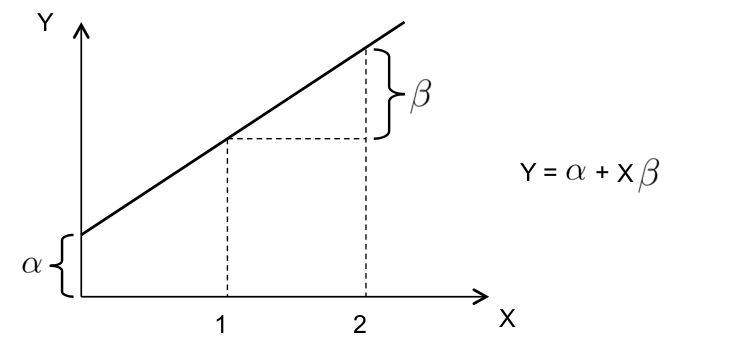
\includegraphics[width=3.5in]{../graphs/linreg}

$\ds{E}[ y ]$ increases by $\beta$ for every unit increase in $x$.
\end{center}
\vskip -1cm
\end{frame}


\begin{frame}


\sk
\begin{columns}[c] 
\column{2in} 
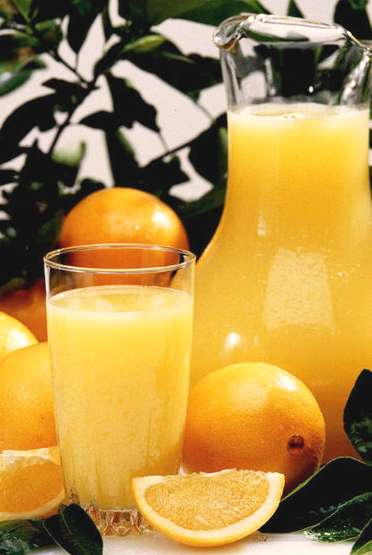
\includegraphics[width=2in]{../graphs/orange-juice}
\column{2in}\small 
\begin{center}

\vskip -1cm
{\bf \Large Orange Juice}

\sk
Three brands ($b$)
{\nv Tropicana, Minute Maid, Dominicks }


\sk 
83 Chicagoland Stores
{\gr Demographic info for each}

\sk
Price, sales (log units moved),  and
whether advertised ({\tt feat}) 

\sk
data in {\tt oj.csv}, code in {\tt oj.R}.
\end{center}

\end{columns} 
\hfill \footnotesize \gr bayesm \& Montgomery, 1987 

\end{frame}


\begin{frame}

{\bf {\nv The Juice:} price, brand, and sales}

\vskip .25cm
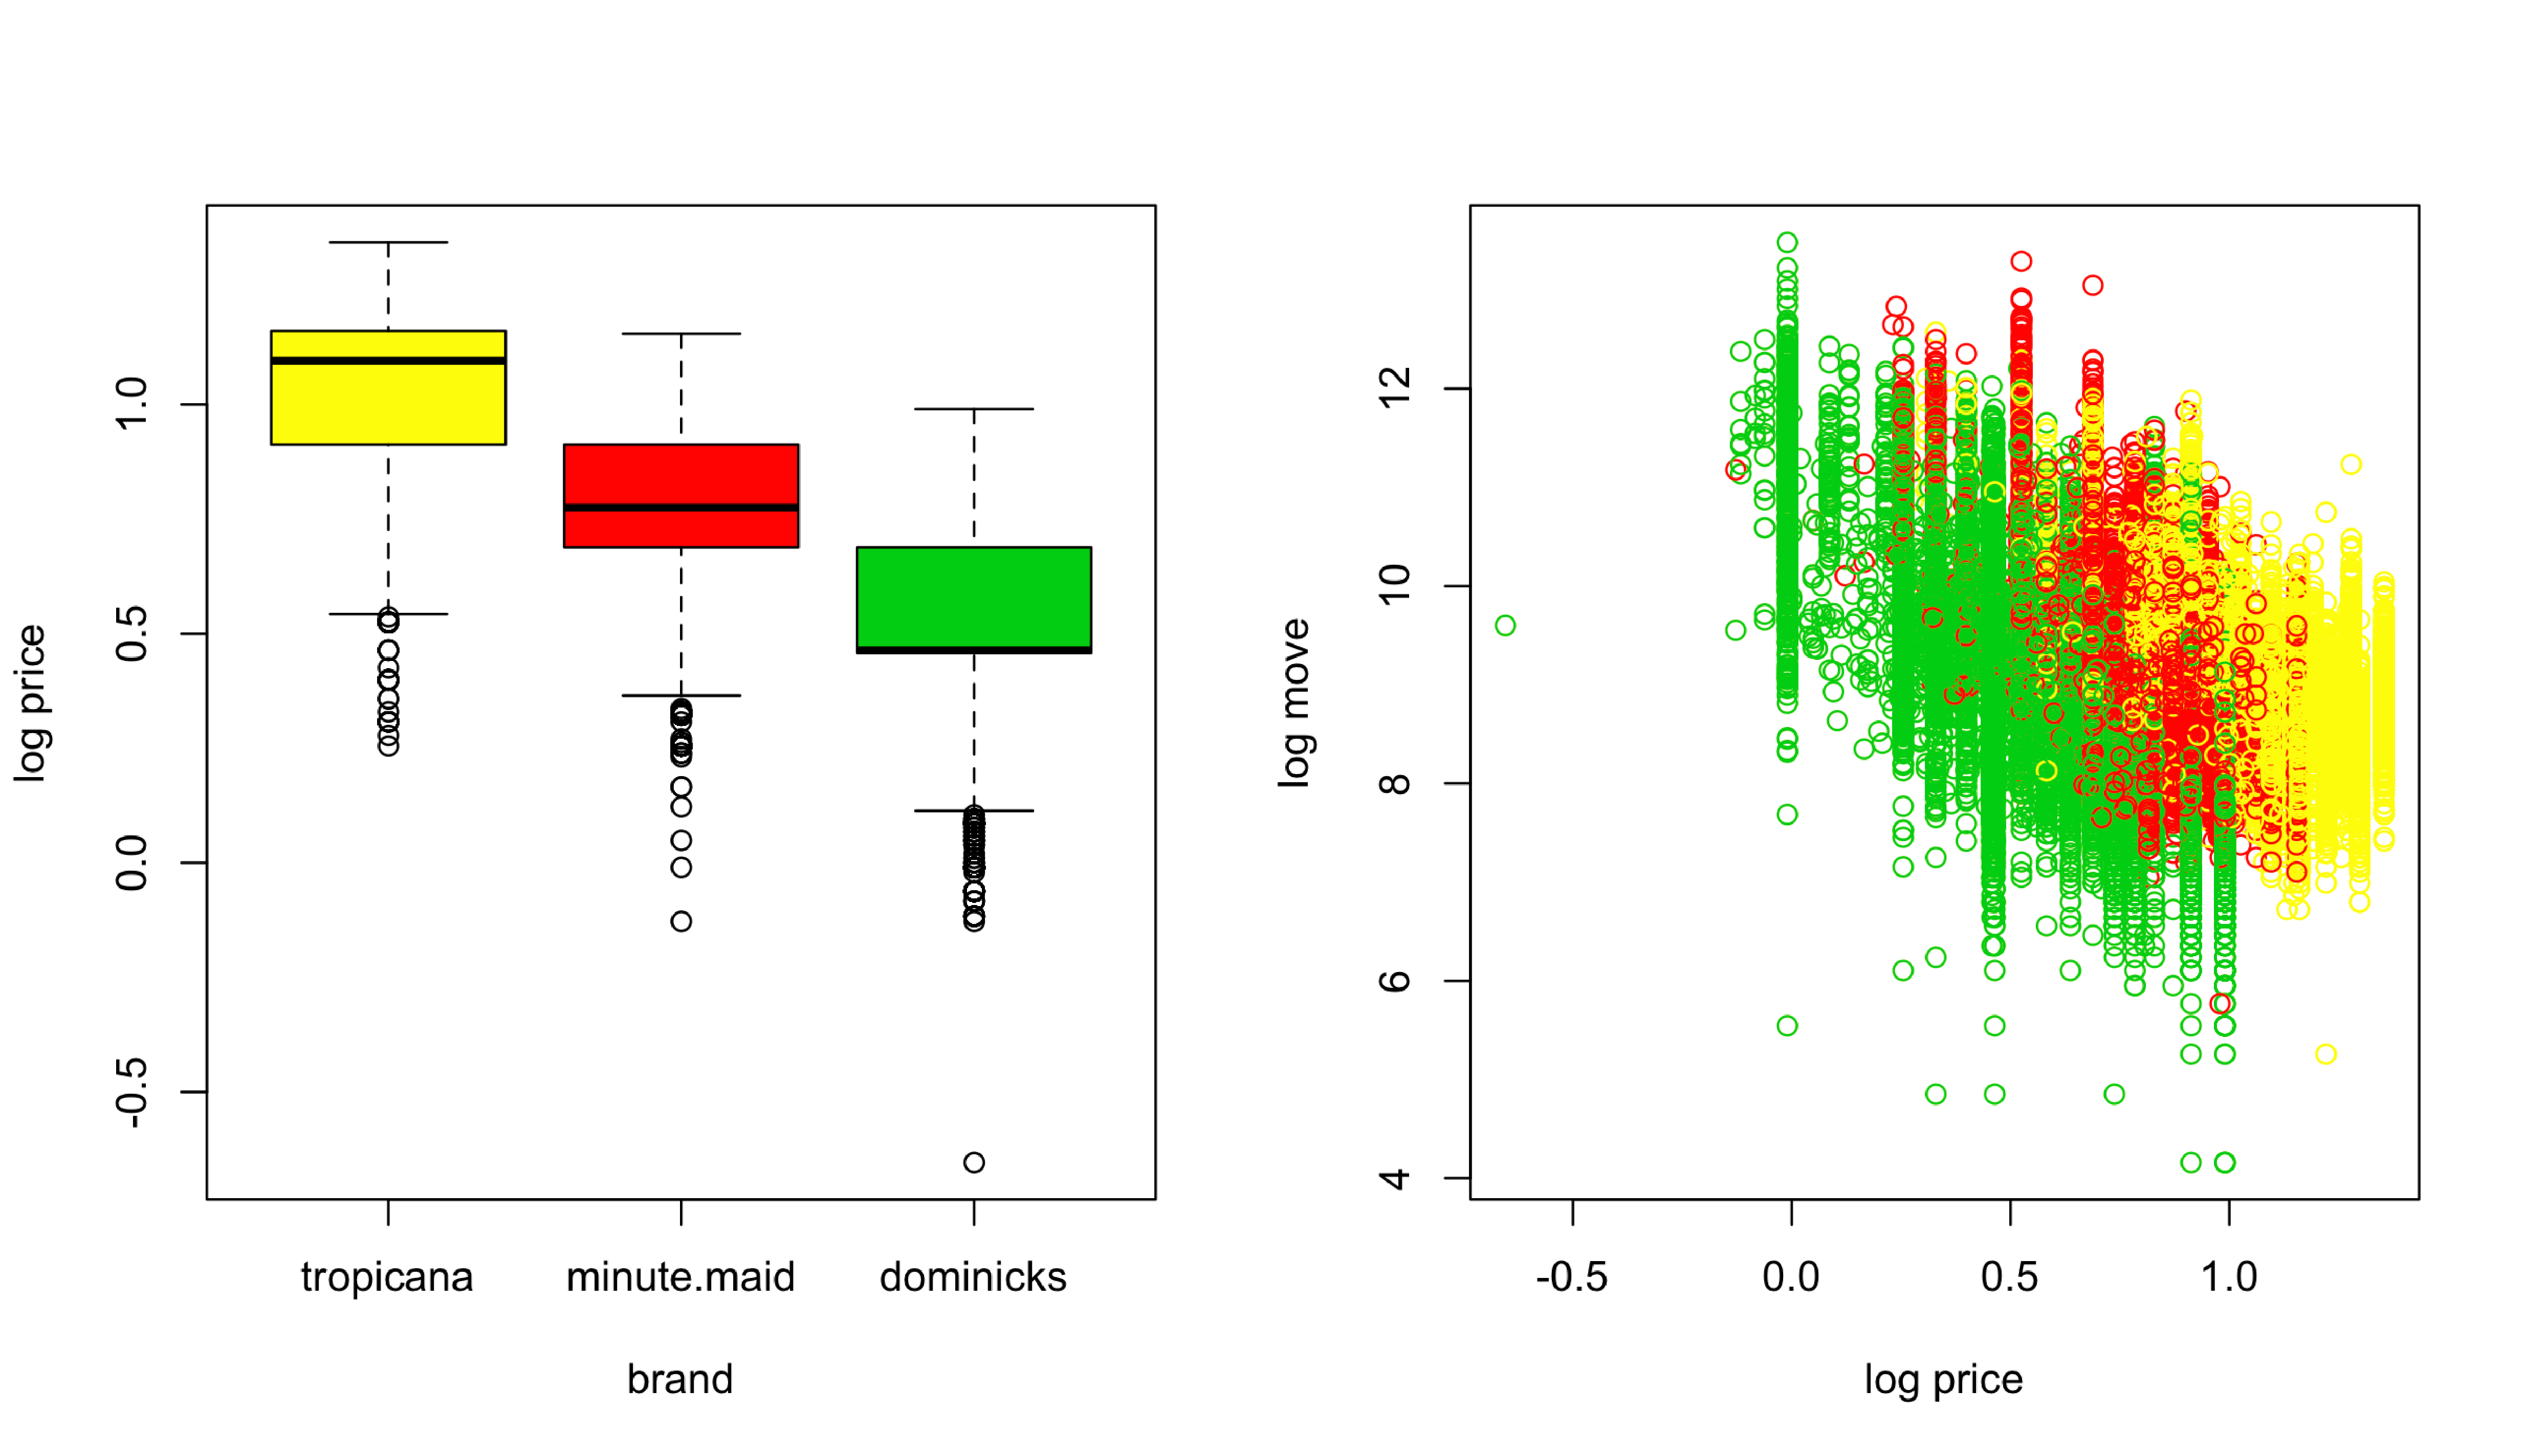
\includegraphics[width=4.3in]{../graphs/OJpriceSmall}

Each brand occupies a well defined price range.\\
Sales decrease with price.
\vskip -.5cm
\end{frame}


\begin{frame}
{Thinking About Scale}

\sk
When making a linear point {\gr (this goes up, that goes down)} think about the scale on which you expect find linearity.

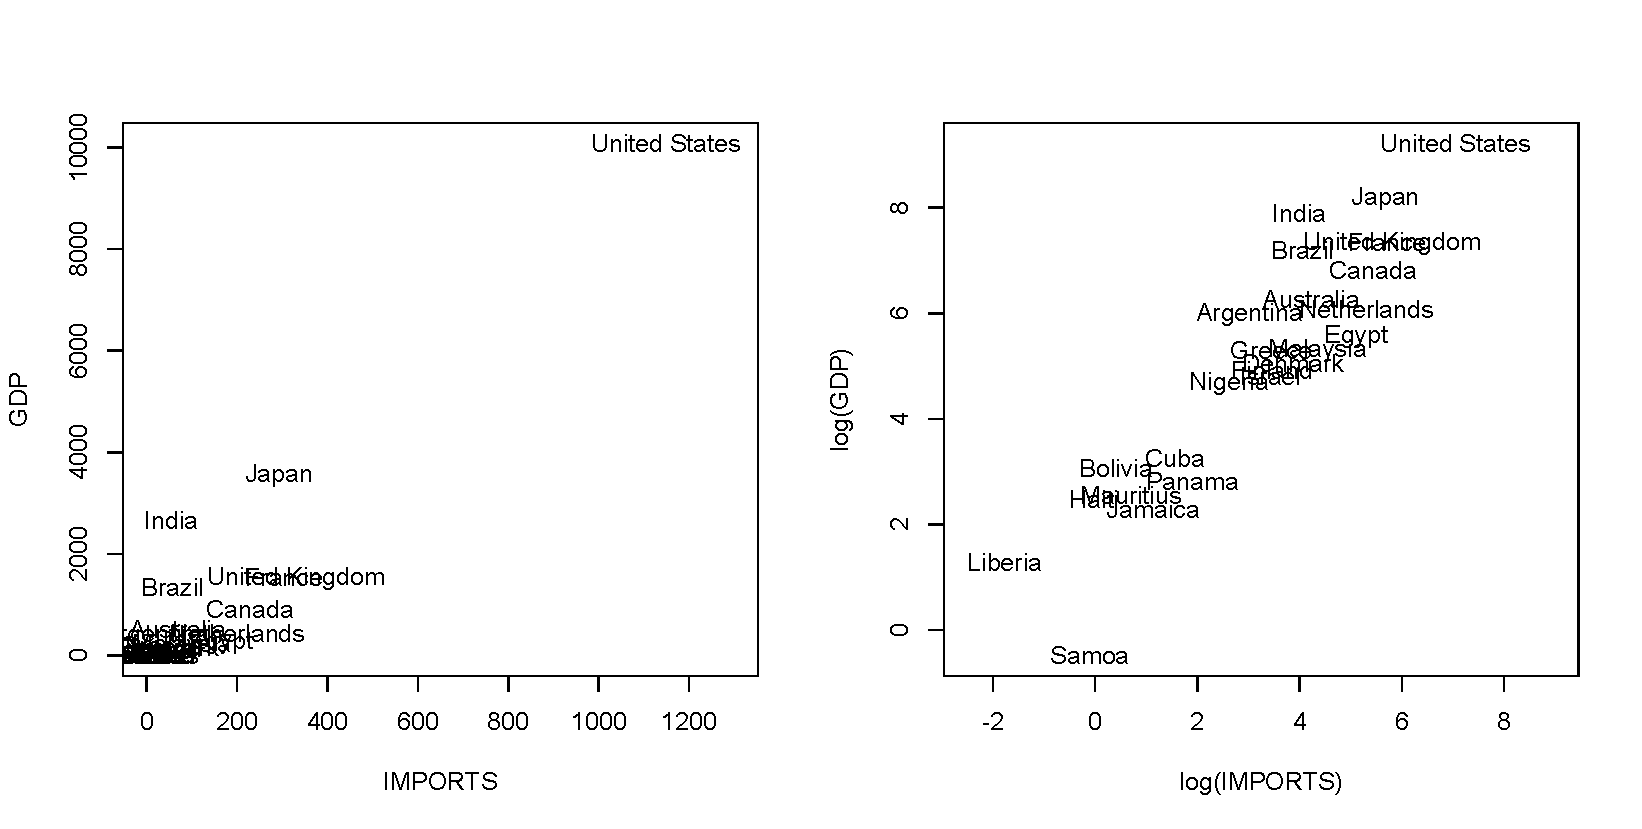
\includegraphics[width=4.2in]{../graphs/trade}

{\sg If your scatterplots look like the left panel, consider using {\theme
    log}.}

\end{frame}


\begin{frame}
{log linear}

We often model the mean for  {\theme log(y)} instead
  of y.


{\theme Why?}    Multiplicative {\gr (rather than additive)} change.

\sk$\log(y) = \log(a) + x\beta \Leftrightarrow
y = ae^{x\beta}$.

\vskip .1cm
Predicted $y$ is multiplied by $e^{\beta}$ after a unit increase in $x$.


\sk
{\gr
Recall that $\log(y) = z \Leftrightarrow e^z=y$ where $e\approx 2.7$ \\
$ \log(ab) = \log(a) + \log(b)$ and
$ \log(a^b) = b\log(a)$.

 I use log=ln, natural log.  Anything else will be noted, e.g., $\log_2$.}


\sk
{\bk Whenever y changes on a percentage scale, use log(y).}\\

\vskip .1cm
prices: {\gr``... Foreclosed homes sell at a 20\% to 30\% discount''}

sales: {\gr``... our y.o.y. sales are up 20\% across models''}

\vskip .1cm
{volatility, fails, rainfall: most things that are strictly positive.}
\end{frame}

\begin{frame}[fragile]
{Price Elasticity}

{A simple orange juice `elasticity model' for sales $y$ has}
\[
\ds{E}[\log y] = \gamma \log({\tt price}) + \bm{x}'\bs{\beta}
\]
{\nv Elasticities and log-log regression:}  for small values we can interpret $\gamma$ as \% change in $y$ per 1\% increase in ${\tt price}$.

\sk
We run this in R:
{\small\vspace{-.5cm}
\begin{semiverbatim}
\nv
\hspace{-.25cm}glm(logmove \til log(price) + brand, data=oj) \sg
\hspace{-.25cm}(Intercept) log(price) branBDinute.maid brandtropicana  
\hspace{-.25cm}    10.8288    -3.1387           0.8702         1.5299  
\end{semiverbatim}}

and see sales drop by about $3.1\%$ for every 1\% price hike.
\vskip -.5cm
\end{frame}

\begin{frame}
{Regression in R}

You need only one command
\begin{center}\vskip -.25cm
\R{ reg = glm(y \til ~var1 + ... + varP, data=mydata) }
\end{center}

\vskip -.25cm
{
\hfill { glm} stands for { Generalized Linear Model}.\\
\hfill {\gr {\tt lm} works too, but {\tt glm} does more.}}

\vskip .25cm
\R{y \til~a + b} is the `formula' that defines your regression.

\R{y\til.} is `regress on every variable in {\tt mydata} not called {\tt y}'

\vskip .25cm

The object \R{reg} is a list of useful things
(type \R{names(reg)}).

\R{ summary(reg)} prints a bunch of information.

\R{ coef(reg)} gives coefficients.

\R{ predict(reg, newdata=mynewdata)} predicts.

\vskip .1cm
{\gr {\tt mynewdata} must be a data frame with exactly the same \\format as {\tt mydata} (same variable names, same factor levels).}

\end{frame}


\begin{frame}[fragile]
{The Design Matrix}

{ What happened to {\tt\theme branddominicks} or {\tt\theme makeDODGE}?}

\vskip .25cm
Our regression formulas look like $\beta_0 + \beta_1x_1 + \beta_2x_2 ...$

But {\tt brand} is not a number, so you can't do {\tt brand}$\times\beta$.

\vskip .25cm
The first step of {\tt glm} is to create a numeric {\it design matrix}.

It does this with a call to the \R{model.matrix} function:
\begin{minipage}[c][.3in]
\begin{verbatim}
"make"
 GMC
 FORD
 DODGE
 FORD
\end{verbatim}
\end{minipage}

{\huge $\Rightarrow$}

\begin{minipage}
\begin{verbatim}
"intercept" "makeFORD" "makeGMC"          
     1           0          1
     1           1          0
     1           0          0
     1           1          0
\end{verbatim}
\end{minipage}

The factor variable is on the left, and on the right we have numeric $x$ that we can multiply against $\bs{\beta}$ coefficients.

\end{frame}

\begin{frame}[fragile]
{Intercepts}


{Our OJ {\tt glm} used {\tt model.matrix} to build a 4 column design:}
\begin{semiverbatim}\small\nv
> x <- model.matrix( \til log(price) + brand, data=oj)
> x[1,] \sg
Intercept log(price) branBDinute.maid brandtropicana 
  1.00000   1.353255         0.000000       1.000000 
\end{semiverbatim}


Each factor's {\theme reference level} is absorbed by the intercept.  
Coefficients are `change relative to reference' (dominicks here).


\vskip .25cm
 To check the reference level of your factors do \\
 \R{levels(myfactor)}  {\gr The first level is reference.}

\vskip .1cm
To change this you can do \\
\R{myfactor = relevel(myfactor, "myref")}.

\end{frame}



\begin{frame}
{Interaction}


Beyond additive effects: { variables change how others act on $y$.}

\sk
An {\theme interaction} term is the product of two covariates,
\[
\ds{E}[~y \mid\bm{x} ~] =  \ldots + \beta_j x_{j} + {\theme x_{j} x_{k}\beta_{jk}}
\]
so that the effect on $\ds{E}[y]$ of a unit increase in $x_j$ is $\beta_j + x_k\beta_{jk}$.

{\theme \hfill It depends upon $x_k$!~~~~~}

\sk
Interactions play a massive role in statistical learning, and they are often central to social science and business questions.
\begin{itemize}
\item Does gender change the effect of education on wages?
\item Do patients recover faster when taking drug A?
\item \nv How does advertisement affect price sensitivity?
\end{itemize}
\vskip -.5cm
\end{frame}


\begin{frame}[fragile]


{\bf {\gr \hspace{-.2cm}Fitting interactions in R:} use * in your formula. } 
\begin{semiverbatim}\small \nv\vspace{-.25cm}
\hspace{-.2cm}glm(logmove \til log(price)*brand, data=oj)\sg
\hspace{-.2cm}Coefficients:
\hspace{-.2cm}                (Intercept)                log(price)  
\hspace{-.2cm}                   10.95468                 {\theme -3.37753}  
\hspace{-.2cm}           branBDinute.maid            brandtropicana  
\hspace{-.2cm}                    0.88825                   0.96239  
\hspace{-.2cm}log(price):branBDinute.maid log(price):brandtropicana  
\hspace{-.2cm}                   {\theme 0.05679                   0.66576}  
\end{semiverbatim}
This is the model $\ds{E}[\log(v)] = \alpha_{b} + \beta_b\log({\tt price})$: 
\\~~a separate intercept and slope for each brand `$b$'.

\sk
Elasticities are\\
~~{\nv dominicks: -3.4},~~ {\theme minute maid: -3.3},~~ {\br tropicana: -2.7}.

{\gr Where do these numbers come from?  Do they make sense?}
\end{frame}


\begin{frame}[fragile]{Advertisements}

{A key question: what changes when we feature a brand?}\\
{\gr Here, this means in-store display promo or flier ad.}

\sk
You could model the additive effect on log sales volume

\vskip .1cm
$\ds{E}[\log({\tt v})] = \alpha_{b} + 
{\theme \ds{1}_{[{\tt feat}]}\alpha_{\tt feat}} + \beta_b\log({\tt p}) $

\vskip .25cm
Or this {\it and} its effect on elasticity
\vskip .1cm
$\ds{E}[\log(v)] = \alpha_{b} + \beta_b\log({\tt p}) + 
{\theme \ds{1}_{[{\tt feat}]}\left(\alpha_{\tt feat} 
+ \beta_{\tt feat}\log({\tt p})\right)}$

\vskip .25cm 
Or its {\it brand-specific} effect on elasticity
\vskip .1cm
$\ds{E}[\log(v)] = \alpha_{b} + \beta_b\log({\tt p}) + 
{\theme \ds{1}_{[{\tt feat}]}\left(\alpha_{b,\tt feat} 
+ \beta_{b,\tt feat}\log({\tt p})\right)}$

\sk
{\gr See the R code for runs of all three models.  \\Connect the regression formula and output to these equations.}

\end{frame}


\begin{frame}

{\bf Brand-specific elasticities}

\begin{center}
\begin{tabular}{l c c c}
& \it Dominicks  & \it Minute Maid & \it Tropicana \\
\it Not Featured & -2.8 & -2.0 & -2.0\\
\it Featured & -3.2 & -3.6 & -3.5\\
\end{tabular}
\end{center}

{\theme Ads always decrease elasticity.  }

\vskip .25cm
Minute Maid and Tropicana elasticities drop 1.5\% with ads,\\ moving them from less to more price sensitive than Dominicks.

\vskip .25cm
{Why does marketing increase price sensitivity?}

{\gr And how does this influence pricing/marketing strategy?}

\end{frame}


\begin{frame}
{Confounding}

\vskip .2cm
Before including {\tt feat}, Minute Maid behaved  like Dominicks.  With {\tt feat}, Minute Maid looks more like Tropicana.  Why?

\vskip .3cm
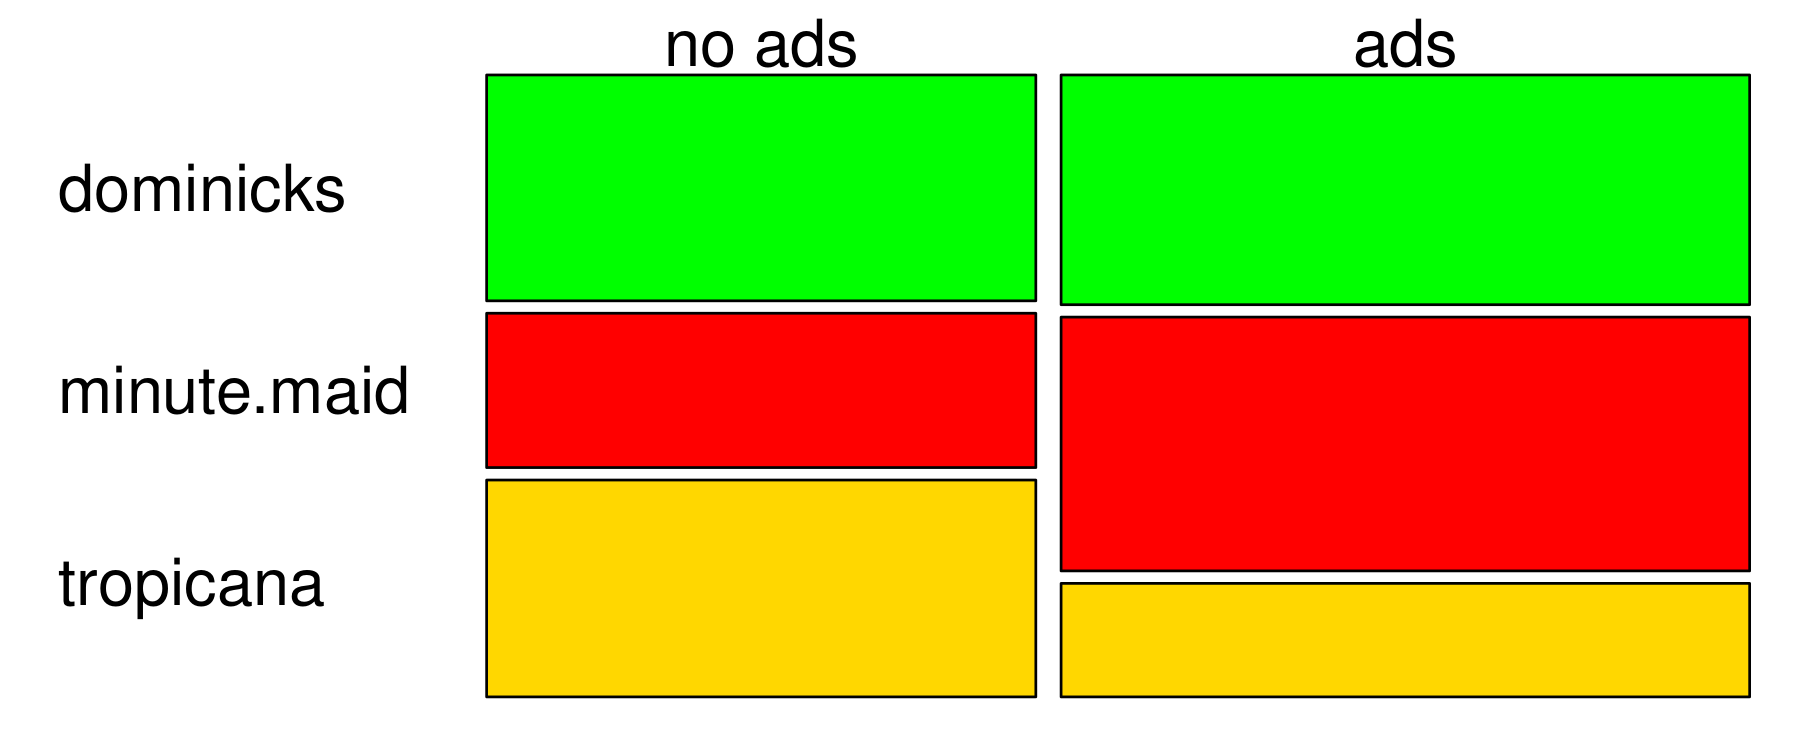
\includegraphics[width=4.25in]{OJsales}

\vskip .25cm
Because Minute Maid was more heavily promoted, and promotions have a negative effect on elasticity, we were {\it confounding} the two effects in the brand average elasticity.
\end{frame}


\begin{frame}
{\theme Logistic Regression}

{Linear regression is just one type of linear model.\\
It is not even the most heavily practiced technique!}

\sk
{\bf Logistic regression: when $\nv \bs{y}$ is {\nv true} or
    {\nv false} {\gr (1/0)}.}

\sk
Binary response as a prediction target:
\begin{itemize}
\item Profit or Loss, greater or less than,  Pay or Default.
\item Thumbs up or down, buy or not buy, potential customer?
\item Win or Lose, Sick or Healthy, Republican or Democrat.
\end{itemize}

\vskip .25cm
In high dimensions, it is often convenient to think binary.

\end{frame}


\begin{frame}

{\bf Building a linear model for \theme binary response data}

\sk
Recall our original model specification: $\ds{E}[~ y \mid \bm{x} ~] =
f( \bm{x}'\bs{\beta} ) $.

\sk
{The response `$\nv y$' is 0 or 1, leading to conditional mean:}
\[
\ds{E}[y | \bm{x}]  ~{\sg = p(y=1 | \bm{x})\times1 + p(y=0 |
  \bm{x})\times0  } ~=  p(y=1 | \bm{x}).
\]
\hfill
$\Rightarrow$ The expectation is a probability.~~~~~~

\sk
We'll choose $f( \bm{x}'\bs{\beta} )$ to
give values between zero and one.

\end{frame}

% pdf("../graphs/logit.pdf",width=6,height=4)
% par(mai=c(1,1,.2,.2))
% x <- seq(-5,5,length=1000)
% plot(x, (1+exp(-x))^{-1}, type="l",bty="n",xlab="XB",ylab="",col=4,lwd=2,yaxt="n",xaxt="n",cex.lab=2)
% text(x=3,y=.75,col=4,label="f(XB)",cex=2)
% abline(v=0, col="grey50",lty=2)
% abline(h=1)
% abline(h=1/2, col="grey50",lty=2)
% axis(2,at=c(0,.5,1),las=1,cex.axis=1.52)
% axis(1,at=c(-5,0,5),cex.axis=1.5)
% dev.off()

\begin{frame}


We want a binary choice model

\vskip -.25cm
\[
p = P(~y=1 \mid \bm{x}~) = f(~\beta_0+\beta_1x_1\ldots+\beta_px_p~)
\]
where $f$ is a function that increases in value from zero to one.

\vskip .25cm
\begin{center}
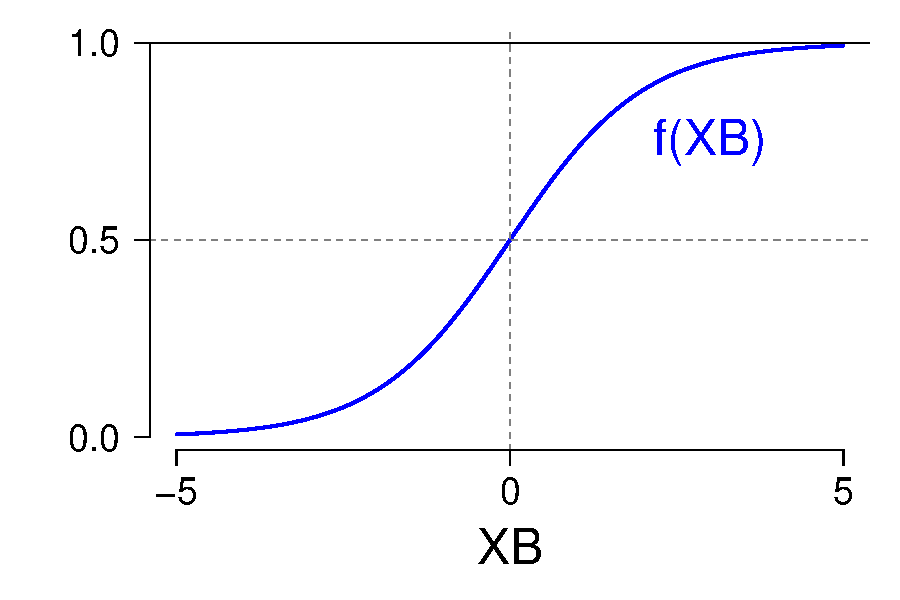
\includegraphics[width=3.25in]{../graphs/logit}
\end{center}
\vskip -.75cm
\end{frame}




\begin{frame}

{\bf We'll use the logit link and do `{\theme logistic regression}'.}

\[
P(y=1 | \bm{x}) =  \frac{e^{\bm{x}'\bs{\beta}}
}{1+e^{\bm{x}'\bs{\beta}}}  = \frac{\exp[\beta_0 + \beta_1x_1\ldots+\beta_dx_d]}
{1+\exp[\beta_0 + \beta_1x_1\ldots+\beta_dx_d]}
\]


\sk
{The `{\nv logit}' link is common, for a couple good
  reasons.}

\sk
One big reason:
A little algebra shows
\[
\log\left[ \frac{p}{1-p} \right] = \beta_0 + \beta_1x_1\ldots+\beta_dx_d,
\]
\hskip 3cm so that it is a linear model for log-odds.

\end{frame}


\begin{frame}
{Spam filter}

\sk
Your inbox does binary regression: {\rd spam} v {\nv not spam}.

{\gr Say $y=1$ for spam, otherwise $y=0$.}

\vskip .25cm
{\tt spam.csv} has for 4600
emails (about 1800 spam) word and character presence indicators (1 if in message) and
related info.

\vskip .25cm
Logistic regression fits $\mr{p}(y=1)$ as a function of
email content.

\vskip .4cm
\begin{adjustwidth}{-.4in}{}
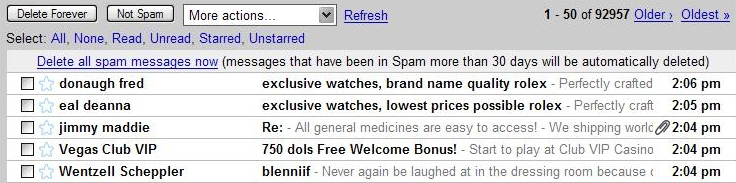
\includegraphics[width=5.05in]{../graphs/SPAMpic}
\end{adjustwidth}

\end{frame}


\begin{frame}

{\bf Logistic regression is easy in R }

\sk{
Again using {\tt glm}:
\begin{center}
\R{glm(Y $\sim$ X, data=mydata, {\theme family=binomial}) }
\end{center}

The argument `{\tt family=binomial}' indicates $y$ is binary.}

\sk
The reponse can take a few forms:
\begin{itemize}
\item $\bm{y} = 1, 1, 0, $ .... numeric vector.
\item $\bm{y} =$ {\tt TRUE, TRUE, FALSE, } .... logical.
\item $\bm{y} =$ {\tt `win',`win',`lose', } .... factor.
%\item $\bm{y} = [1,0], [1,0], [0,1], $ .... numeric matrix.
\end{itemize}
\vskip .2cm
 Everything else is the same as for linear regression.

\end{frame}

\begin{frame}[fragile]
{Perfect Separation}

\begin{semiverbatim}\nv\footnotesize
spammy <- glm(spam\til., data=email, family='binomial')\rd
Warning message:
glm.fit: fitted probabilities numerically 0 or 1 occurred 
\end{semiverbatim}

We're warned that some emails are clearly spam or not spam.

\vskip .1cm
This is called `{\nv perfect separation}'.  You don't need to worry.

\vskip .1cm
The situation can introduce numeric instability in your algorithm (mess with standard errors, p-values, etc), but is largely benign.

\vskip .25cm
It occurs here because some words are clear {\nv discriminators}:
\begin{semiverbatim}\nv
email\$word_george>0\bk          
                    FALSE TRUE
          important  2016  772
          spam       1805    8
\end{semiverbatim}
Guy's named George; spammers in the early 90s weren't fancy.
\end{frame}

\begin{frame}[fragile]
{Interpreting Coefficients}

{The model is 
\[
\frac{p}{1-p} = \exp\left[ \beta_0 + x_1\beta_1 \ldots x_p\beta_p \right]
\]
So $\exp(\beta_j)$ is the {\theme odds multiplier} for a unit increase in $x_j$.}

\vskip .25cm
{\tt b["word\_george"]=-5.8}, so {\tt george} in an email multiplies  odds of spam by $\exp(-5.8) \approx 0.003$.

\vskip .25cm
{\tt b["char\_dollar"]=1.9}, so having `{\tt \$}' in an email multiplies  odds of spam by $\exp(1.9) \approx 6.5$.

\vskip .25cm
What is the odds multiplier for a covariate coefficient of zero?
\end{frame}


\begin{frame}[fragile]

{The summary function gives coefficients, plus some other info.}

The bit at the bottom is especially useful:

\begin{semiverbatim}\footnotesize
\nv{summary(spammy)}\br ...
(Dispersion parameter for binomial family taken to be 1)
    Null deviance: 6170.2  on 4600  degrees of freedom
Residual deviance: 1548.7  on 4543  degrees of freedom
AIC: 1664.7
\end{semiverbatim}

The same stuff is in output for our {\it linear} OJ regression.
\begin{semiverbatim}\footnotesize
\nv{summary(ojreg)}\br ...
(Dispersion parameter for gaussian family taken to be 0.48)
    Null deviance: 30079  on 28946  degrees of freedom
Residual deviance: 13975  on 28935  degrees of freedom
AIC: 61094
\end{semiverbatim}

These are stats on fit, and they are important in either linear or logistic regression.  Understanding {\theme deviance} ties it all together.
\end{frame}



\begin{frame}
{Estimation and Fit}

{\bf Two complementary concepts: }

\sk
{{\theme Deviance} refers to the distance between data and fit.}\\
{ You want to make it as small as possible.}

\vskip .25cm
{{\theme Likelihood} is the probability of your data given parameters.} \\
{ You want to make it as big as possible.}

\begin{center}\large
\nv Deviance = {\large -}2log[
  Likelihood ] {\gr + C} 
\end{center}
\hfill{\gr C is a constant you can mostly ignore.}

\sk
We'll think of deviance as a cost to be minimized.

This is referred to as maximum likelihood estimation (MLE)

\end{frame}


\begin{frame}

{\bf  Least-Squares and deviance in \nv linear regression}

\sk
The probability model is $y \sim \mr{N}(\bm{x}'\bs{\beta} ,\sigma^2)$.

\vskip .2cm
{\gr $N(\mu, \sigma^2)=\exp\left[-(y-\mu)^2/2\sigma^2\right]/\sqrt{2\pi\sigma^2}.$}

\sk

Given $n$  independent observations, 
the likelihood is 
\[
\prod_{i=1}^n \mr{pr}(y_i | \bm{x}_i) 
= \prod_{i=1}^n \mr{N}( y_i ; 
\bm{x}_i'\bs{\beta}, \sigma^2  ) \propto \exp\left[ -\frac{1}{2}\sum_{i=1}^n \left( y_i  - 
\bm{x}_i'\bs{\beta}\right)^2/\sigma^2 \right]
\]




This leads to Deviance $\displaystyle \propto
\frac{1}{\sigma^2} \sum_{i=1}^n \left( y_i  - 
\bm{x}_i'\bs{\beta}\right)^2$.

\vskip .25cm 
{\theme Minimizing deviance is the same as least squares!}

{\gr And thus the MLE minimizes our sum of squared errors.}

\end{frame}



\begin{frame}
{\theme MLE for Logistic Regression}

\vskip .25cm
Our logistic regression likelihood is the product
\begin{eqnarray*}\vspace{-.2cm}
\text{LHD} &=& \prod_{i=1}^n P(y_i | \bm{x}_i) =  \prod_{i=1}^n p_i^{y_i}
(1-p_i)^{1-y_i}\\
&&\hspace{-.75cm}   =
\prod_{i=1}^n\left(\frac{\exp[\bm{x}_i'\bs{\beta}]}
{1+\exp[\bm{x}_i'\bs{\beta}]}\right)^{y_i}
\left(\frac{1}
{1+\exp[\bm{x}_i'\bs{\beta}]}\right)^{1-y_i}
\end{eqnarray*}

This is maximized by minimizing the deviance
\begin{align*}
D &= -2\sum_{i=1}^n\left( y_i \log(p_i) + (1-y_i) \log(1-p_i)
\right)\\
&\nv \propto \sum_{i=1}^n\left[  
\log\left(1 + e^{\bm{x}_i'\bs{\beta}}\right) 
- y_i \bm{x}_i'\bs{\beta}\right]
\end{align*}
\gr All we've done is take the logarithm and multiply by $-2$.

\end{frame}


\begin{frame}[fragile]

{We have the same output as for a linear/gaussian model.}

\vskip .25cm
But the `{\tt dispersion parameter}' here is always set to one.

{\gr Check this to make sure you've actually run logistic regression. }

{\footnotesize 
\begin{semiverbatim}\nv
> summary(spammy)\br...
(Dispersion parameter for binomial family taken to be 1)
    Null deviance: 6170.2  on 4600  degrees of freedom
Residual deviance: 1815.8  on 4543  degrees of freedom
AIC: 1931.8
\end{semiverbatim}}

`{\theme degrees of freedom}' is actually `number of observations - df',
where df is the number of coefficients estimated in the model.

\vskip .1cm
That is, {\nv df(deviance) = nobs - df(regression).}

\vskip .1cm
From the R output, how many observations do we have?  
\end{frame}


\begin{frame}[fragile]

{\bf Sum of Squares (Deviance) is the bit we need to minimize: }
\[ D \propto \sum_{i=1}^n \left( y_i  - 
\bm{x}_i\bs{\beta}\right)^2
\]
This makes the observed data {\it as likely as possible}.

\sk
 {Error variance  $\sigma^2$ measures variability
  around the mean. }\\
{i.e., $\sigma^2 = \mr{var}(\varepsilon)$, where $\varepsilon_i = y_i - 
\bm{x}_i\bs{\beta}$ are the `{\nv residuals}'.}\\

\vskip .25cm
{ R estimates $\sigma^2$ and calls it the {\tt \theme dispersion parameter}.}

e.g., in output for our linear OJ regression:
\begin{semiverbatim}\footnotesize \br\vspace{-.5cm}
\hspace{-.25cm}(Dispersion parameter for gaussian family taken to be 0.48)
\end{semiverbatim}
Even if we know $\bs{\beta}$, we  only predict log sales {\it with uncertainty}.  \\e.g., there's a 95\% probability of log sales in $\bm{x}'\bs{\beta} \pm 2\sqrt{0.48}$
\end{frame}

\begin{frame}

\sk
{\theme Residual} deviance $D$ is what we've minimized, using $\bm{x}'\bs{\beta}$.

\vskip .1cm
{\theme Null} deviance $D_0$ is for the model where you don't use
$\bm{x}$.\\
i.e., if you use $\hat y_i = \bar y$:
\begin{itemize}
\item $D_0 = \sum (y_i - \bar{y})^2$ in linear regression.
\item $D_0 = -2\sum\left[ y_i\log(\bar{y}) + (1-y_i)\log(1-\bar{y})\right]$ in logistic reg.
\end{itemize}

\sk
{\bf The difference between $D$ and $D_0$ is due to info in
$\bm{x}$.}

\vskip .25cm
Proportion of deviance explained by $\bm{x}$ is called $R^2$:
\[
R^2 = \frac{D_0 -D}{D_0} = 1 - \frac{D}{D_0}.
\]
This measures how much variablity you are able to model.

\vskip .25cm
~~~in {\tt spammy}: ~~$R^2 = 1 - 1549/6170 = 0.75$\\
~~~in {\tt ojreg}: ~~$R^2 = 1 - 13975/30079 = 0.54$
\end{frame}



\begin{frame}[fragile]
{$R^2$ in linear regression}

{These forumulas should look pretty familiar.}

\vskip .25cm
$R^2 = 1 - $ SSE/SST from previous classes, \\and linear deviance is just the Sum of Squares!

\vskip .25cm
You'll also recall that $R^2 = \mr{cor}(y,\hat y)^2$ in linear regression, \\where $\hat y$ denotes `fitted value' $\hat y = f(\bm{x}'\bs{\hat\beta}) 
\gr = \bm{x}'\bs{\hat\beta}$ {\gr in lin reg.}
\begin{semiverbatim}\nv
cor(ojreg\$fitted,oj\$logmove)^2\br
[1] 0.5353939
\end{semiverbatim}
For linear regression, min deviance = max $\mr{cor}(y,
  \hat{y})$.

  {\gr If $y$ vs $\hat y$ makes a straight line, you have a perfect
  fit.}
\end{frame}

\begin{frame}
{Fit plots: $\hat y$ vs $y$}

\begin{center}
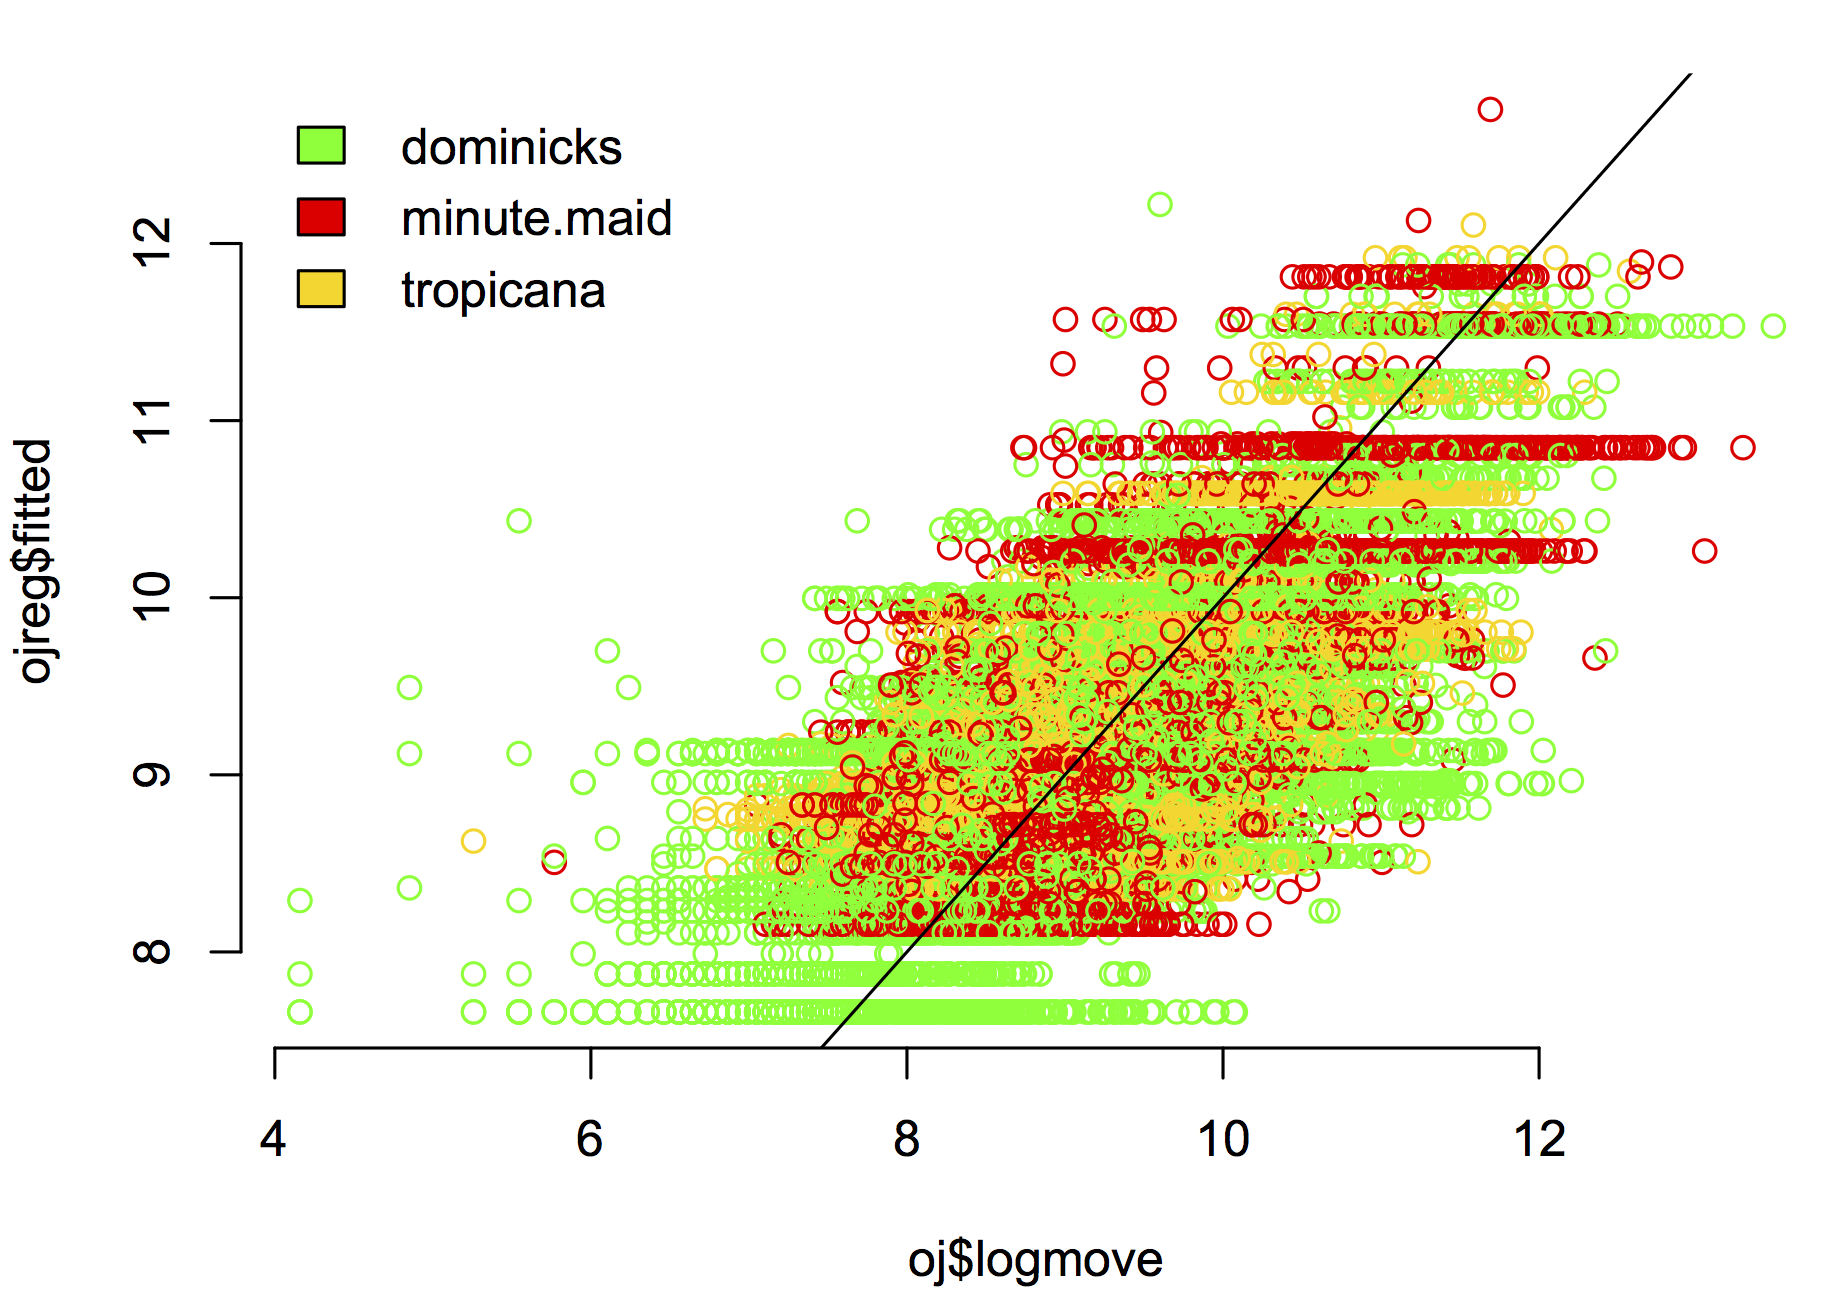
\includegraphics[width=3.55in]{ojfit}
\end{center}

It's good practice to plot $\hat y$ vs $y$ as a check for mispecification. \gr (e.g., non-constant variance, nonlinearity in residuals, ...)
\end{frame}


\begin{frame}
{Fit plots for logistic regression}

{We can plot $\hat y$ vs $y$ in logistic regression using a boxplot.}

\begin{center}
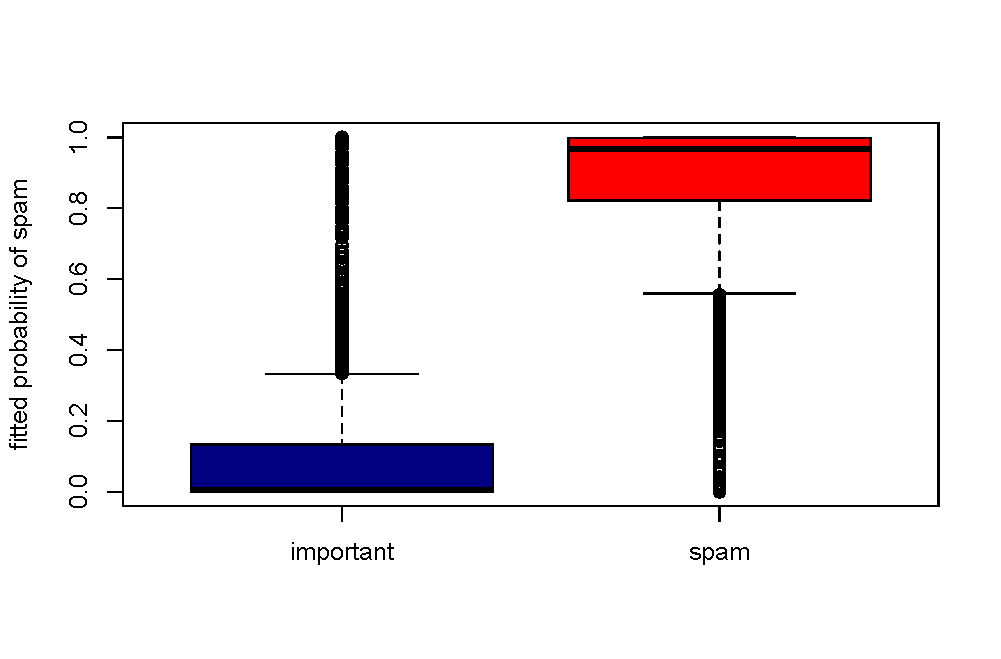
\includegraphics[width=3.75in]{spamfit}
\end{center}

{The estimation pushes each distribution away from the middle.}\\
\gr Where would you choose for a classification cut-off?
\end{frame}



\begin{frame}[fragile]
{Prediction}

{We've seen that prediction is easy with {\tt glm}:}
\begin{semiverbatim}\small \nv\vspace{-.5cm}
predict(spammy, newdata=email[1:4,])\br
      1          2         3         4 
2.029963 10.956507 10.034045  5.656989 
 \end{semiverbatim}
This outputs $\bm{x}'\bs{\hat\beta}$ for each $\bm{x}$ row of {\tt mynewdata}.

\sk
In logistic regression, to get { probabilities} $e^{\bm{x}'\bs{\hat\beta}}/(1+e^{\bm{x}'\bs{\hat\beta}})$,\\ add the argument 
{ \tt type="response"}.
\begin{semiverbatim}\small \nv\vspace{-.5cm}
predict(spammy, newdata=email[1:4,], type="response")\br
        1         2         3         4 
0.8839073 0.9999826 0.9999561 0.9965191
\end{semiverbatim}


{\gr {\tt newdata} {\it must} match the format of original data.}

\end{frame}


\begin{frame}[fragile]
{Out-of-Sample Prediction}

{You care about how your model predicts out-of-sample (OOS).}

\vskip .25cm
One way to test this is to use a validation sample.

~~Fit your model to the remaining {\it training data}, \\~~and see how well it predicts the {\it left-out data}.

\begin{semiverbatim}\footnotesize
\gr# Sample 1000 random indices \nv
leaveout <- sample(1:nrow(email), 1000)
\gr# train the model WITHOUT these observations \nv
spamtrain <- glm(spam\til., 
              data=email[-leaveout,], family='binomial')
\gr# predicted probability of spam on the left out data \nv
pspam <- predict(spamtrain, 
              newdata=email[leaveout,], type='response')
\end{semiverbatim}

\end{frame}

\begin{frame}
{Out-of-Sample Prediction}

Fit plots on the 1000 left out observations.

\vskip .25cm
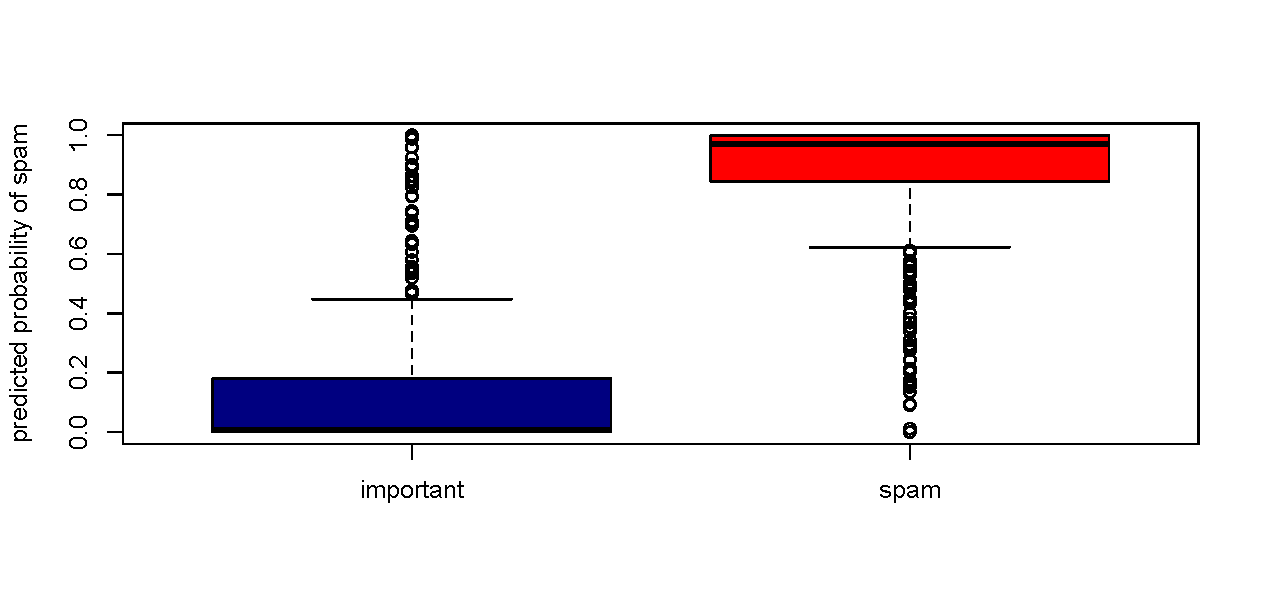
\includegraphics[width=4.25in]{pspam}

\vskip .25cm

{\tt deviance.R} has a function to get deviances from {\tt y} and {\tt pred}.

\vskip .1cm
For the left-out data, we get $D0 = 1332$, $D=562$, $R^2=0.58$.

\vskip .1cm
{\gr Since the sample is random, you might get different results.}

\vskip .25cm
{\theme Note: OOS $R^2$ is lower than in-sample $R^2$ ($> 0.75$).}



\end{frame}


\begin{frame}
{Week 2 Homework}

{\bf{\theme American Housing Survey}: 2004 home values}
\begin{columns}[c]
\column{3in}

\sk
~~~~
\includegraphics[width=3in]{../graphs/salesign}
\column{1in}\small
\begin{center}

\sg Demographics\\
{\gr School, Income}

\vskip .25cm
Finance \\
{\gr Mortgage, Sale}

\vskip .25cm
Neighborhood\\
{\gr Noise, Smells}

\vskip .25cm
Geography
{\gr State, Urban?}
\end{center}
\end{columns}

\end{frame}


\begin{frame}

We'll be modelling $\log$ home value, and whether or not the buyer had at least 20\% down  {\gr (when I grabbed this data, \\there was lots of talk about stricter mortgage requirements).} 

\sk
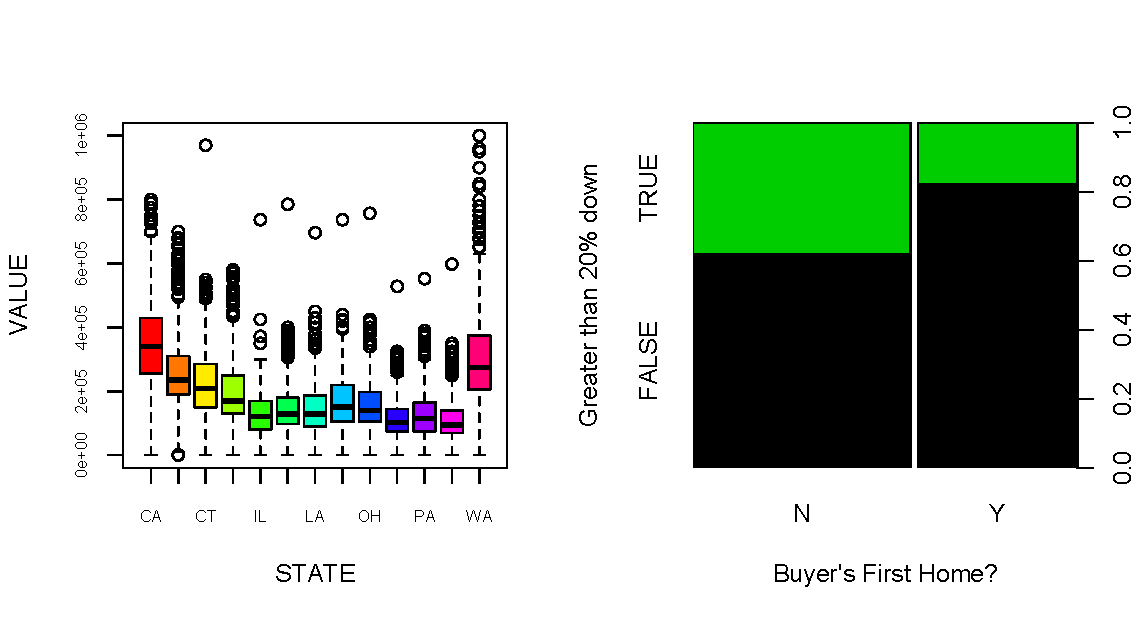
\includegraphics[width=4.25in]{homesintro}

\vskip .25cm
Data is in {\tt homes2004.csv}, with variable dictionary in {\tt homes2004code.txt}.  Primer is in {\tt homes2004\_start.R}.

\vskip -.5cm

\end{frame}

\begin{frame}
{Week 2 Homework}

[1] Plot some relationships and tell a story.

\vskip .25cm
[2] Regress log value onto all but mortgage and purchase \$.  
\begin{itemize}
\item How many coefficients are significant at 10\% FDR?
\item Re-run regression with only the significant covariates,\\ and compare $R^2$ to the full model.
\end{itemize}

\vskip .25cm
[3] Fit a regression for whether the buyer had $\geq 20\%$ down (again, onto everything but {\tt AMMORT} and {\tt LPRICE}).  
\begin{itemize}
\item Interpret effects for 1st home buyers and \# of bathrooms.
\item Add + describe interaction for 1st home-buyers and \#baths. 
\end{itemize}

\vskip .25cm
[4] Re-fit your model from Q3 for only homes worth 
$>100k$.  Compare in-sample fit to $R^2$ for predicting homes worth $<\!100k$.


\end{frame}

\end{document}
